%-----------------------------------------------------------------------------%
% Packages & Other Configurations
%-----------------------------------------------------------------------------%
\RequirePackage{fix-cm}  % Fix Font shape `OT1/cmr/m/n' size substitution.
\documentclass[a4paper,10pt]{article}
\usepackage[top=0.3in, bottom=0.3in, left=1in, right=0.9in]{geometry}
\usepackage[utf8]{inputenc} %add acents
\usepackage{setspace} % command \doublespacing etc...
\usepackage{lineno} % number lines
\usepackage{epsf,epsfig} % includegraphics [pdf, png etc]
\usepackage{amsmath} %adicionei esse pacote pra vc poder usar o draft%
\usepackage{textcomp} %símbolos de texto
\usepackage{natbib} % bibtex - adicionar referencia
\usepackage{multicol}
% \usepackage{url} % for bibtex - configuracoes de urls
\usepackage{tabularx} % for tables
\usepackage[hidelinks]{hyperref}  % Add URL links.
% \usepackage[bookmarks=false,colorlinks=true,urlcolor={green},linkcolor={green},pdfstartview={XYZ null null 1.22}]{hyperref} %all references
\usepackage{tikz}
\usepackage{lscape}
\usepackage{siunitx}
\usepackage{geometry}

%-----------------------------------------------------------------------------%
% Adicionar a Watermark
%-----------------------------------------------------------------------------%
\usepackage{draftwatermark}
\SetWatermarkAngle{45}
\SetWatermarkLightness{0.9}
\SetWatermarkFontSize{5cm}
\SetWatermarkScale{0.3}
\SetWatermarkText{Prática 4 - Oceanografia}
%-----------------------------------------------------------------------------%
% Informações sobre o PDF
%-----------------------------------------------------------------------------%
\pdfinfo{%
  /Title    (GEO232 - Prática 4)
  /Author   (Ju Leonel)
  /Creator  (Ju Leonel)
  /Producer (Ju Leonel)
  /Subject  (Intro oceanografias)
  /Keywords (Intro oceanografia, prática 4)}

%-----------------------------------------------------------------------------%
% Documento
%-----------------------------------------------------------------------------%
\title{GEO232 - Introdução à Oceanografia - Prática 4}
\author{\vspace{-10ex}}
\date{\vspace{-10ex}}

\geometry{hmargin=1cm,vmargin=1cm}

\begin{document}
 \maketitle
 \phantom{}

1. A tabela abaixo lista a temperatura e a salinidade de uma estação oceanográfica oceânica situada no sul da Califórnia.

\begin{center}
  \begin{tabular}{|c|c|c|c|c|c|}
    \hline
    Profundidade    & Temperatura    & Salinidade           & Produndidade    & Temperatura    & Salinidade \\
    (m) & (\textcelsius) & (\textperthousand) & (m) & (\textcelsius) & (\textperthousand) \\
      0      & 14.56          & 31.22              & 250      & 6.57           & 33.98 \\
     10      & 14.50          & 31.40              & 300      & 6.15           & 34.01 \\
     20      & 14.48          & 31.56              & 400      & 5.49           & 34.07 \\
     30      & 12.72          & 31.88              & 500      & 4.01           & 34.14 \\
     50      & 10.86          & 32.40              & 600      & 4.65           & 34.20 \\
     75      &  9.20          & 33.24              & 700      & 4.36           & 34.26 \\
    100      &  8.82          & 33.60              & 800      & 4.10           & 34.31 \\
    150      &  7.77          & 33.88              & 1000     & 3.51           & 34.41 \\
    200      &  7.10          & 33.94              &          &                &  \\
    \hline
  \end{tabular}
\end{center}

\def\width{4}
\def\hauteur{10}

\begin{multicols}{2}
  \begin{center}
    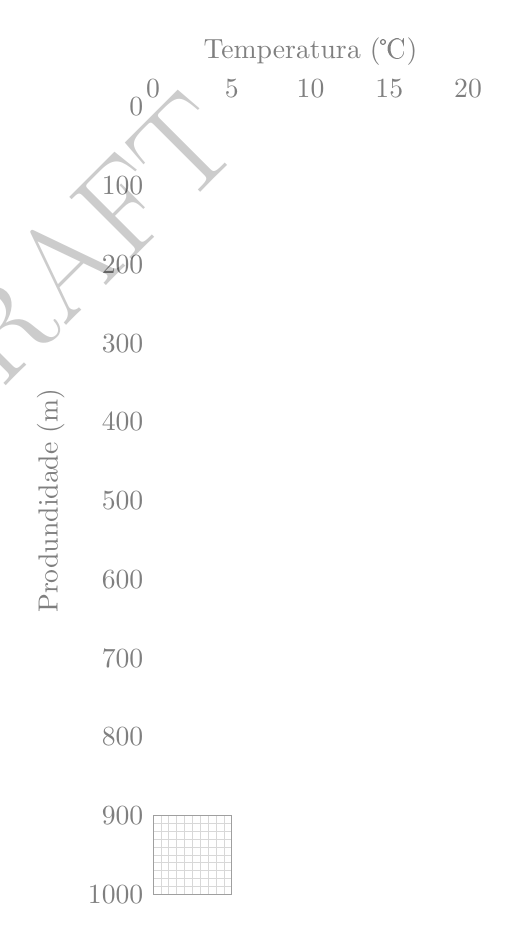
\begin{tikzpicture}[x=10mm, y=10mm, semitransparent]
    % Grid.
    \draw[xstep=10mm, ystep=10mm, line width=0.1mm, black!90!white] (0,0) grid (\width,\hauteur);
    \draw[step=1mm, line width=0.1mm, black!30!white] (0,0) grid (\width,\hauteur);
    % x-tickslabels.
    \draw[black] ( 0, 10) node[anchor=south] {0};
    \draw[black] ( 1, 10) node[anchor=south] {5};
    \draw[black] ( 2, 10) node[anchor=south] {10};
    \draw[black] ( 3, 10) node[anchor=south] {15};
    \draw[black] ( 4, 10) node[anchor=south] {20};
    % x-labels.
    \draw[black] (2, 11) node[anchor=north] {Temperatura (\textcelsius)};
    % y-labels.
    \draw[black] (-1, 5) node[anchor=south, rotate=90] {Produndidade (m)};
    % y-tickslabels left.
    \draw[black] (0, 10) node[anchor=east] {0};
    \draw[black] (0, 9) node[anchor=east] {100};
    \draw[black] (0, 8) node[anchor=east] {200};
    \draw[black] (0, 7) node[anchor=east] {300};
    \draw[black] (0, 6) node[anchor=east] {400};
    \draw[black] (0, 5) node[anchor=east] {500};
    \draw[black] (0, 4) node[anchor=east] {600};
    \draw[black] (0, 3) node[anchor=east] {700};
    \draw[black] (0, 2) node[anchor=east] {800};
    \draw[black] (0, 1) node[anchor=east] {900};
    \draw[black] (0, 0) node[anchor=east] {1000};
    \end{tikzpicture}
  \end{center}

\columnbreak

  \begin{center}
    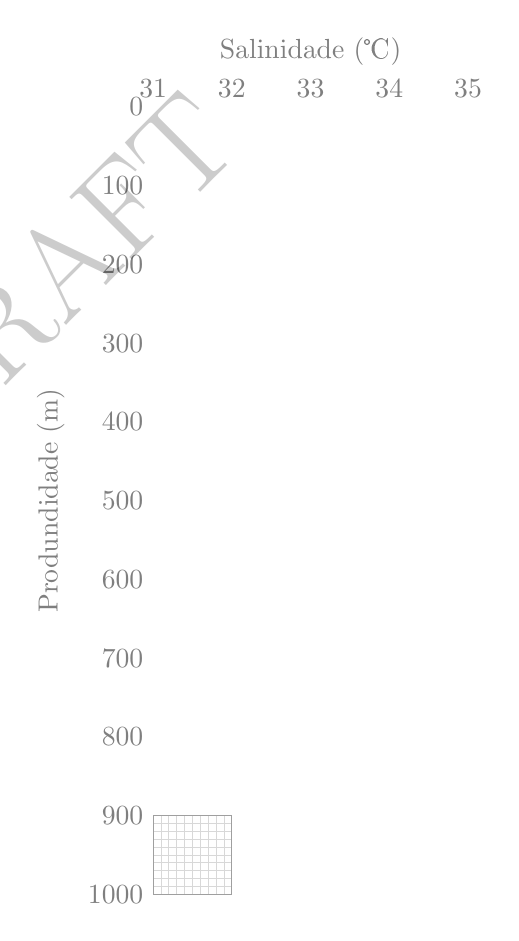
\begin{tikzpicture}[x=10mm, y=10mm, semitransparent]
    % Grid.
    \draw[xstep=10mm, ystep=10mm, line width=0.1mm, black!90!white] (0,0) grid (\width,\hauteur);
    \draw[step=1mm, line width=0.1mm, black!30!white] (0,0) grid (\width,\hauteur);
    % x-tickslabels.
    \draw[black] ( 0, 10) node[anchor=south] {31};
    \draw[black] ( 1, 10) node[anchor=south] {32};
    \draw[black] ( 2, 10) node[anchor=south] {33};
    \draw[black] ( 3, 10) node[anchor=south] {34};
    \draw[black] ( 4, 10) node[anchor=south] {35};
    % x-labels.
    \draw[black] (2, 11) node[anchor=north] {Salinidade (\textcelsius)};
    % y-labels.
    \draw[black] (-1, 5) node[anchor=south, rotate=90] {Produndidade (m)};
    % y-tickslabels left.
    \draw[black] (0, 10) node[anchor=east] {0};
    \draw[black] (0, 9) node[anchor=east] {100};
    \draw[black] (0, 8) node[anchor=east] {200};
    \draw[black] (0, 7) node[anchor=east] {300};
    \draw[black] (0, 6) node[anchor=east] {400};
    \draw[black] (0, 5) node[anchor=east] {500};
    \draw[black] (0, 4) node[anchor=east] {600};
    \draw[black] (0, 3) node[anchor=east] {700};
    \draw[black] (0, 2) node[anchor=east] {800};
    \draw[black] (0, 1) node[anchor=east] {900};
    \draw[black] (0, 0) node[anchor=east] {1000};
    \end{tikzpicture}
  \end{center}
\end{multicols}

\begin{itemize}
  \item[(a)] Grafique os valores de temperatura em função da profundidade;
  \item[(b)] Grafique os valores de salinidade em função da profundidade;
  \item[(c)] Descreva os perfis encontrados. Sugiro motivos pelos quais a variação de temperatura é maior nas camadas mais superficiais.
  \end{itemize}

\end{document}
